\documentclass[10pt]{article}
\usepackage[margin=2cm]{geometry}
\usepackage{amsmath,amssymb}
\usepackage{float}
\usepackage{graphicx,booktabs,multirow,caption}
\usepackage{stfloats} % o \usepackage{dblfloatfix}
\begin{document}

\section*{Análisis Comparativo de Algoritmos Evolutivos}

En este apartado se presentan los resultados obtenidos al evaluar diferentes algoritmos (Firefly (30\% reubicación de población), ACOR (15\% reubicación de población para soluciones cercanas), Algoritmo Genético Diploide y PSO con división de población) sobre un conjunto de benchmarks dinámicos. Los resultados se analizaron considerando calidad y adaptabilidad.

\subsection*{Métricas de Evaluación}

El rendimiento de los algoritmos se midió a través de métricas clave como lo son \emph{calidad} y \emph{adaptabilidad}, seleccionadas por su relevancia en la comparación de algoritmos evolutivos en entornos dinámicos. Diversos autores coinciden en que estas métricas permiten analizar no sólo el desempeño estático, sino también la capacidad de recuperación ante cambios \cite{morrison2003performance}.

\textbf{Calidad}: El desempeño se cuantificó mediante las métricas \textit{Avg Best Pre-Change}, \textit{Avg Avg Pre-Change} y \textit{Avg Worst Pre-Change}, que representan respectivamente la mejor, promedio y peor solución encontrada antes de la modificación del entorno. En entornos dinámicos, la calidad es un indicador esencial para evaluar la robustez de un algoritmo, pues refleja su capacidad para mantenerse cercano al óptimo incluso frente a perturbaciones \cite{ahmed2024adaptive,morrison2003performance}. Además, la literatura en optimización evolutiva dinámica reconoce que las medidas de desempeño basadas en mejores, peores y promedios de fitness son criterios habituales de evaluación en benchmarks dinámicos \cite{nguyen2012survey,weicker2003performance}.

\textbf{Adaptabilidad}: La velocidad de adaptación se midió con la métrica \textit{Avg Recovery Iter}, que indica el número promedio de iteraciones que tarda el algoritmo en recuperar un nivel competitivo de desempeño tras un cambio ambiental. Un valor bajo en esta métrica sugiere una alta capacidad de respuesta. En este sentido, Ahmed \cite{ahmed2024adaptive} propone un marco adaptativo basado en detección y reajuste dinámico, mientras que Nguyen et al. \cite{nguyen2013kd} y Weicker \cite{weicker2003performance} destacan que un algoritmo competitivo no sólo debe encontrar soluciones de calidad, sino también reaccionar rápidamente a los cambios en el entorno.

Estas métricas combinadas permiten una evaluación integral del desempeño algorítmico: mientras que la calidad garantiza soluciones eficaces, la adaptabilidad mide la capacidad de respuesta frente al dinamismo del entorno, facilitando comparaciones más completas entre distintos enfoques evolutivos en problemas no estacionarios \cite{morrison2003performance}.

\subsection*{Resultados}

A continuación se muestra un extracto de los resultados obtenidos para cada algoritmo. 

% --- FIREfly ---
\subsubsection*{Firefly (30\% reubicación de población)}
\begin{table}[H]
\centering
\caption{Resultados del algoritmo FireFly (30\% reubicación de población en cambio).}
\label{tab:firefly}
\scriptsize
\begin{tabular}{lcccccc}
\toprule
\textbf{Benchmark} & \textbf{Avg Best Pre-Change} & \textbf{Avg Avg Pre-Change} & \textbf{Avg Worst Pre-Change} & \textbf{Avg Std Pre-Change} & \textbf{Avg Recovery Iter} & \textbf{Avg Time (s)} \\
\midrule
1 & 4.326799 & 4.651963 & 4.936076 & 0.303534 & 6.00 & 21.6962 \\
2 & 0.000020 & 0.001634 & 0.008346 & 0.002818 & 2.00 & 142.5533 \\
3 & 1.949308 & 10.796254 & 19.559685 & 7.103091 & 7.00 & 44.1845 \\
4 & 0.009526 & 0.350470 & 1.574578 & 0.533295 & 3.00 & 8.6900 \\
5 & -307.245057 & -210.955552 & -124.780520 & 56.984993 & 9.00 & 16.2412 \\
\bottomrule
\end{tabular}
\end{table}

En el benchmark 1, el algoritmo  (30\% reubicación de población) mostró un mejor valor promedio previo al cambio de 4.326799 y un peor valor de 4.936076. La desviación estándar fue relativamente baja (0.303534) y el algoritmo necesitó 6 iteraciones para recuperarse tras los cambios en el entorno.

En el benchmark 2 alcanzó valores muy cercanos a cero en todas las métricas de calidad (con un mejor valor de 0.000020 y un peor valor de 0.008346). La recuperación fue rápida (2 iteraciones).

En el benchmark 3, el mejor valor alcanzado fue de 1.949308, mientras que el peor ascendió a 19.559685. La desviación estándar fue alta (7.103091), lo que indica cambios relevantes entre ejecuciones. El algoritmo tardó 7 iteraciones en recuperarse.

El benchmark 4 mostró un mejor valor promedio de 0.009526 y el peor de 1.574578, con una desviación estándar de 0.533295,  la recuperación fue relativamente rápida (3 iteraciones).

Por último, en el benchmark 5 se observaron valores negativos, con un mejor resultado de -307.245057 y un peor de -124.780520 con una desviación estándar de 56.984993, lo que muestra alta dispersión en los resultados, la recuperación requirió 9 iteraciones.

% --- ACOR ---
\subsubsection*{ACOR (15\% reubicación para soluciones cercanas)}
\begin{table}[H]
\centering
\caption{Resultados del algoritmo ACOR (15\% reubicación de población para soluciones cercanas).}
\label{tab:acor}
\scriptsize
\begin{tabular}{lcccccc}
\toprule
\textbf{Benchmark} & \textbf{Avg Best Pre-Change} & \textbf{Avg Avg Pre-Change} & \textbf{Avg Worst Pre-Change} & \textbf{Avg Std Pre-Change} & \textbf{Avg Recovery Iter} & \textbf{Avg Time (s)} \\
\midrule
1 & 4.322080 & 4.636836 & 4.936076 & 0.315635 & 4.00 & 21.4260 \\
2 & 0.000003 & 0.000812 & 0.004291 & 0.001482 & 2.00 & 229.7759 \\
3 & 0.615696 & 7.753642 & 16.017607 & 6.289126 & 5.00 & 45.0635 \\
4 & 0.208088 & 1.371044 & 4.142520 & 1.240571 & 4.00 & 8.2121 \\
5 & -372.732798 & -283.084570 & -196.890480 & 56.532546 & 12.00 & 16.4673 \\
\bottomrule
\end{tabular}
\end{table}

Con base a lo mostrado en la tabla 2 del algoritmo ACOR (15\% reubicación de población para soluciones cercanas) se observa que en el benchmark 1, el algoritmo alcanzó un valor promedio mínimo previo al cambio de 4.322080, mientras que el promedio general fue de 4.636836 y el peor caso se situó en 4.936076. La desviación estándar fue baja (0.315635), lo que refleja un comportamiento estable y con poca dispersión entre las ejecuciones. La recuperación se logró en 4 iteraciones, lo que muestra una capacidad aceptable de adaptación.

En el benchmark 2, los resultados fueron muy cercanos a cero, con un mejor valor de 0.000003 y un peor valor de 0.004291. Esto evidencia una gran precisión en la solución encontrada. La desviación estándar también fue pequeña (0.001482), confirmando la consistencia en los resultados. Además, la recuperación fue rápida, logrando estabilizarse en solo 2 iteraciones.

Mientras que en el benchmark 3 el mejor valor alcanzado fue 0.615696, mientras que el peor se elevó hasta 16.017607, con un promedio de 7.753642. La desviación estándar fue alta (6.289126), lo que indica que el algoritmo presentó cambios relevantes en la calidad de las soluciones. La recuperación se completó en promedio en 5 iteraciones, mostrando una adaptación moderada.

Durante el benchmark 4, un mejor valor fue de 0.208088 y un peor caso de 4.142520, mientras que el promedio se situó en 1.371044. La desviación estándar fue relativamente elevada (1.240571). La recuperación ocurrió en 4 iteraciones.

Finalmente, en el benchmark 5, se registraron valores negativos, con un mejor caso de -372.732798 y un peor de -196.890480, mientras que el promedio fue de -283.084570. La dispersión de los resultados fue considerable, con una desviación estándar de 56.532546, lo que indica alta variabilidad, el algoritmo requirió 12 iteraciones para recuperarse, lo cual indica que la adaptación fue más lenta en este escenario en comparación con los otros benchmarks.


% --- Genético Diploide ---
\subsubsection*{Algoritmo Genético Diploide}
\begin{table}[H]
\centering
\caption{Resultados del algoritmo Genético Diploide.}
\label{tab:ga-diploid}
\scriptsize
\begin{tabular}{lcccccc}
\toprule
\textbf{Benchmark} & \textbf{Avg Best Pre-Change} & \textbf{Avg Avg Pre-Change} & \textbf{Avg Worst Pre-Change} & \textbf{Avg Std Pre-Change} & \textbf{Avg Recovery Iter} & \textbf{Avg Time (s)} \\
\midrule
1 & 0.000000 & 0.035916 & 0.358191 & 0.113236 & 1.00 & 23.1954 \\
2 & 0.000000 & 0.000002 & 0.000012 & 0.000005 & 1.00 & 261.8552 \\
3 & 0.118543 & 0.120936 & 0.126520 & 0.003853 & 1.00 & 46.4383 \\
4 & 0.049361 & 0.062799 & 0.075962 & 0.011708 & 1.00 & 10.1156 \\
5 & -365.078117 & -336.985790 & -241.255015 & 42.507788 & 3.00 & 17.9002 \\
\bottomrule
\end{tabular}
\end{table}

Podemos observar que el algoritmo logra en el benchmark 1 un desempeño muy cercano al óptimo, alcanzando un valor mínimo promedio de 0.000000, con un promedio general de 0.035916 y un peor caso de 0.358191. La desviación estándar fue baja (0.113236), lo que indica estabilidad en los resultados. La recuperación se logró en solo 1 iteración, teniendo una gran capacidad de adaptación.

Pero en el benchmark 2, los valores obtenidos fueron muy pequeños, con un mejor resultado de 0.000000, un promedio de 0.000002 y un peor caso de apenas 0.000012. La desviación estándar fue mínima (0.000005). El algoritmo recuperó su desempeño en una sola iteración.

En el benchmark 3, se alcanzó un mejor valor de 0.118543, con un promedio muy cercano de 0.120936 y un peor resultado de 0.126520. La baja desviación estándar (0.003853) confirma la estabilidad del algoritmo en este escenario. Se volvio a dar una recuperación en una sola iteración, lo que subraya su rapidez de adaptación.

Lo que sucede en el benchmark 4, se muestra en la tabla que el mejor caso fue de 0.049361, el promedio de 0.062799 y el peor de 0.075962. La desviación estándar fue de 0.011708, manteniéndose baja y mostrando un buen control de la variabilidad. La recuperación se efectuó en solo 1 iteración como ocurrio en los benchmarks pasados.

Por último, en el benchmark 5, los valores fueron negativos, con un mejor desempeño de -365.078117 y un peor resultado de -241.255015, mientras que el promedio se dio en -336.985790. La desviación estándar fue considerablemente más alta (42.507788), mientras que la recuperación fue un poco más lenta en comparación con los demás casos, requiriendo 3 iteraciones.



% --- PSO dividido ---
\subsubsection*{PSO con división de población}
\begin{table}[H]
\centering
\caption{Resultados del algoritmo PSO con división de población.}
\label{tab:pso-dividido}
\scriptsize
\begin{tabular}{lcccccc}
\toprule
\textbf{Benchmark} & \textbf{Avg Best Pre-Change} & \textbf{Avg Avg Pre-Change} & \textbf{Avg Worst Pre-Change} & \textbf{Avg Std Pre-Change} & \textbf{Avg Recovery Iter} & \textbf{Avg Time (s)} \\
\midrule
1 & 5.943962 & 7.390896 & 10.005467 & 1.278012 & 3.00 & 20.9818 \\
2 & 0.000070 & 0.014321 & 0.072558 & 0.023924 & 4.00 & 203.1267 \\
3 & 3.451031 & 11.693936 & 18.890177 & 5.933817 & 8.00 & 44.6182 \\
4 & 0.676358 & 2.349877 & 5.216153 & 1.387639 & 4.00 & 8.3659 \\
5 & -325.050923 & -231.300190 & -152.200474 & 54.129551 & 7.00 & 16.3406 \\
\bottomrule
\end{tabular}
\end{table}

Con base a lo presentado en la tabla podemos observar como en el benchmark 1, el PSO con división de población alcanzó valores relativamente altos, con un mejor desempeño de 5.943962 y un peor caso de 10.005467 con una desviación estándar de 1.278012 mientras que la adaptación fue rápida con 3 iteraciones.

En el caso del benchmark 2, los valores obtenidos fueron más pequeños. El mejor caso se acercó a cero (0.000070), aunque la media (0.014321) y el peor caso (0.072558), reflejada en una desviación estándar de 0.023924, esto nos indica que el algoritmo no siempre produce soluciones consistentes en este escenario por otro lado la recuperación tomó 4 iteraciones.

El benchmark 3 tenemos el mejor resultado de 3.451031, pero el promedio subió a 11.693936, y en el peor caso se llegó a 18.890177 por otro lado podemos observar que tenemos una desviación estándar alta (5.933817), lo que deja ver que el rendimiento varió entre ejecuciones, para este caso se requirio 8 iteraciones para la adaptación.

En el benchmark 4, el mejor valor (0.676358) se mantuvo bajo, aunque el promedio (2.349877) y el peor resultado (5.216153) mientras que la variabilidad (1.387639) y la recuperación se completó en 4 iteraciones, manteniendo un nivel de adaptabilidad aceptable.

Por ultimo en el benchmark 5 mostró valores negativos, teniendo el mejor caso en -325.050923, el promedio en -231.300190 y el peor en -152.200474, en este caso la recuperación fue más lenta que en los otros benchmarks con 7 iteraciones en promedio.

\subsection*{Discusión Comparativa}

En términos de calidad, el Algoritmo Genético Diploide se posiciona como el más destacado ya que presenta valores promedio prácticamente en cero en varios benchmarks (por ejemplo, 0.000002 en el Benchmark 2 y 0.1209 en el Benchmark 3), lo que indica soluciones muy cercanas al óptimo. Cabe mencionar que sus mejores valores (Best) alcanzan el desempeño esperado, lo que significa que logra encontrar el óptimo en ciertos escenarios. Este resultado coincide con lo planteado por Nguyen et al. \cite{nguyen2012survey} y Weicker \cite{weicker2003performance}, quienes subrayan que la calidad debe evaluarse considerando tanto el mejor como el promedio y el peor desempeño para capturar una visión global en entornos dinámicos.

Por otra parte, algoritmos como PSO con división de población presentan promedios significativamente más altos (7.39 en el Benchmark 1 y 11.69 en el Benchmark 3), reflejando soluciones de menor calidad; en cambio, Firefly (30\% reubicación de población) y ACOR (15\% reubicación de población para soluciones cercanas) se sitúan en un punto intermedio, alcanzando resultados aceptables pero con mayor dispersión. Esto respalda lo señalado por Weicker \cite{weicker2003performance}, quien enfatiza que la calidad no puede analizarse de forma aislada, sino vinculada a la estabilidad y consistencia de los resultados.

Respecto a la adaptabilidad, se confirma la ventaja del Genético Diploide, ya que en casi todos los casos logra recuperarse en una sola iteración tras un cambio, evidenciando una población capaz de reaccionar de manera inmediata. Este hallazgo es coherente con Ahmed \cite{ahmed2024adaptive} y Nguyen et al. \cite{nguyen2013kd}, quienes remarcan que la capacidad de reajustarse rápidamente tras un cambio es esencial para mantener la competitividad en problemas dinámicos. Por contraste, Firefly (30\% reubicación de población) y ACOR (15\% reubicación de población para soluciones cercanas) requieren entre 2 y 6 iteraciones y el PSO con división de población hasta 8, lo que indica una respuesta más lenta. Estos resultados coinciden con lo señalado por Weicker \cite{weicker2003performance}, quien advierte que ciertos mecanismos de diversidad pueden no garantizar una recuperación eficiente.

Tomando en cuenta calidad y adaptabilidad, el Algoritmo Genético Diploide es el más competitivo, ya que logra soluciones de alta calidad junto con una recuperación inmediata. En el extremo opuesto, PSO con división de población resulta menos adecuado por su calidad deficiente y lenta capacidad de respuesta, mientras que Firefly (30\% reubicación de población) y ACOR (15\% reubicación de población para soluciones cercanas) representan enfoques intermedios, con un balance aceptable aunque menos consistente.



\subsection*{Resultados Gráficos}

A continuación, se presentan algunas gráficas que nos permiten visualizar de forma comparativa el desempeño de los algoritmos en términos de iteraciones de recuperación y valores de calidad pre-cambio.

\begin{figure}[H]
    \centering
    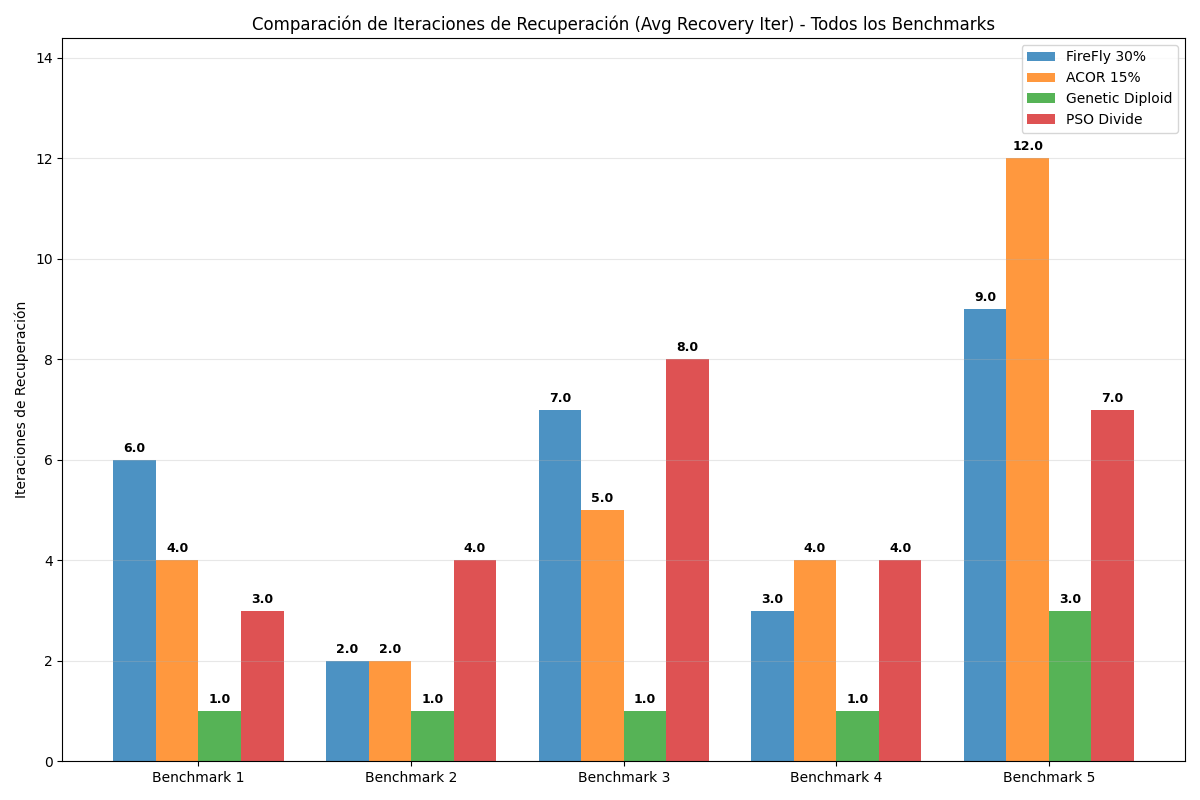
\includegraphics[width=0.95\textwidth]{imagenes/iteraciones.png}
    \caption{Comparación de Iteraciones de Recuperación (Avg Recovery Iter) para todos los benchmarks.}
    \label{fig:recuperacion}
\end{figure}

\begin{figure}[H]
    \centering
    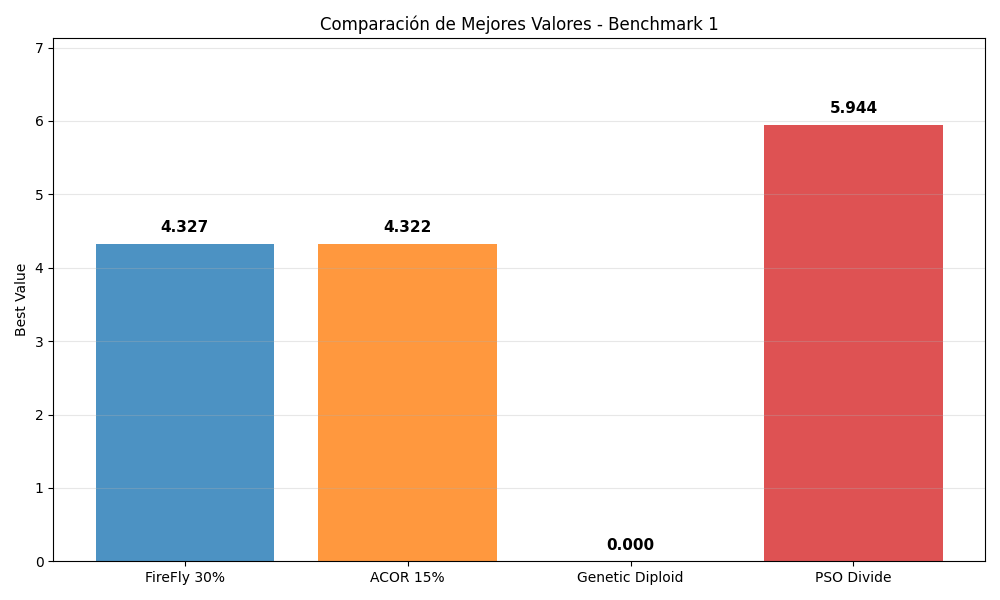
\includegraphics[width=0.8\textwidth]{imagenes/b1.png}
    \caption{Comparación de Mejores Valores Pre-Cambio (Avg Best Pre-Change) en el Benchmark 1.}
    \label{fig:b1}
\end{figure}

\begin{figure}[H]
    \centering
    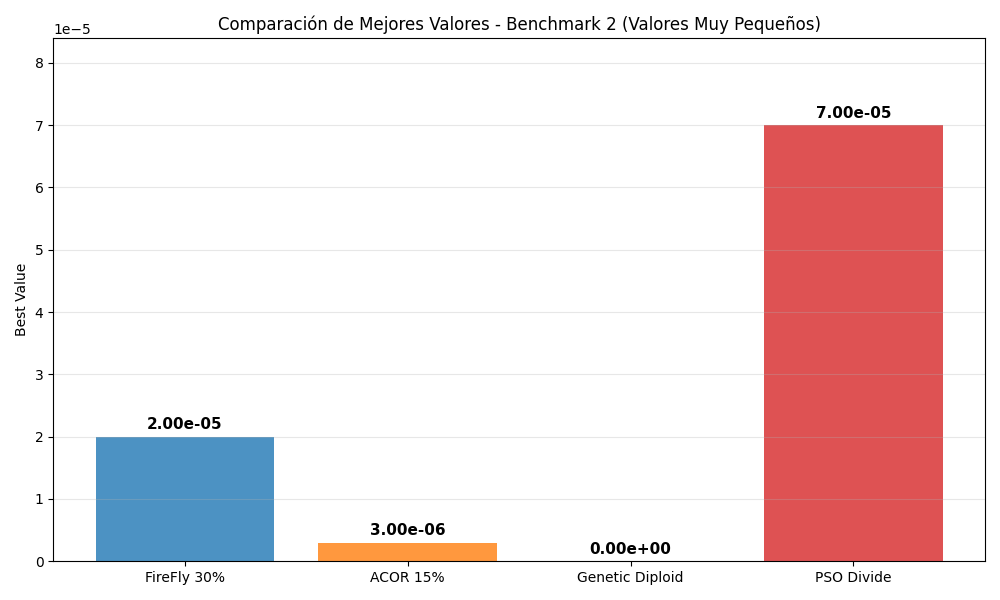
\includegraphics[width=0.8\textwidth]{imagenes/b2.png}
    \caption{Comparación de Mejores Valores Pre-Cambio (Avg Best Pre-Change) en el Benchmark 2 (valores muy pequeños).}
    \label{fig:b2}
\end{figure}

\begin{figure}[H]
    \centering
    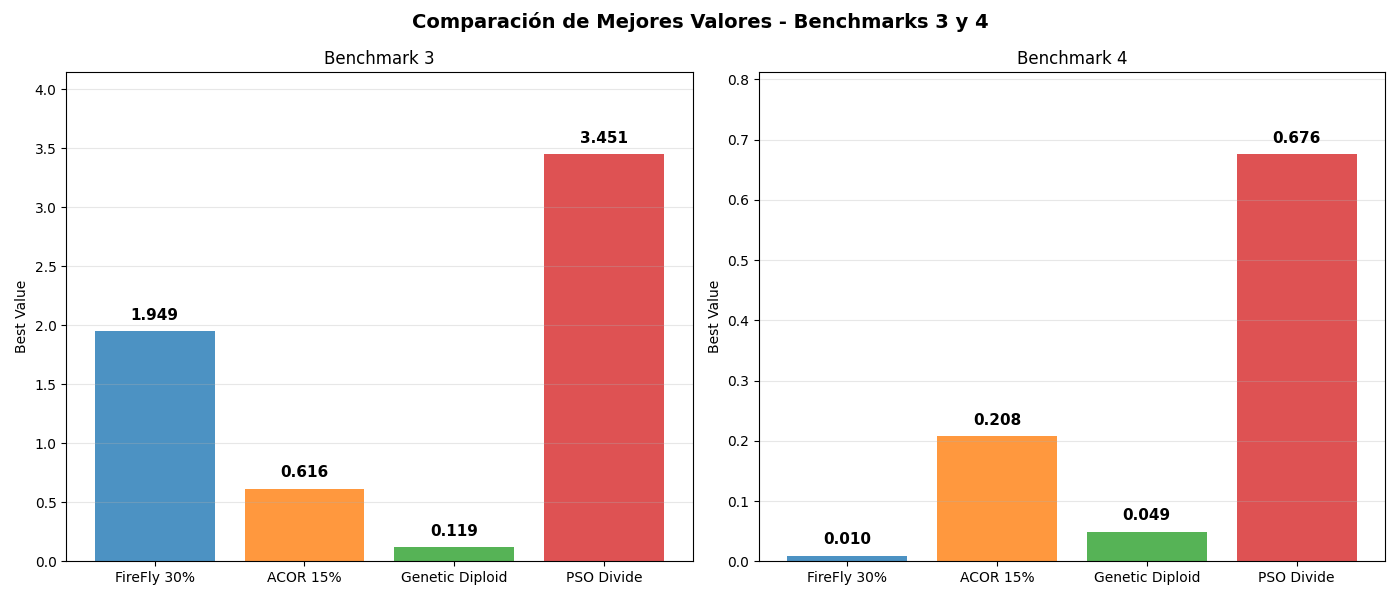
\includegraphics[width=0.95\textwidth]{imagenes/b3_y_b4.png}
    \caption{Comparación de Mejores Valores Pre-Cambio en los Benchmarks 3 y 4.}
    \label{fig:b3b4}
\end{figure}

\begin{figure}[H]
    \centering
    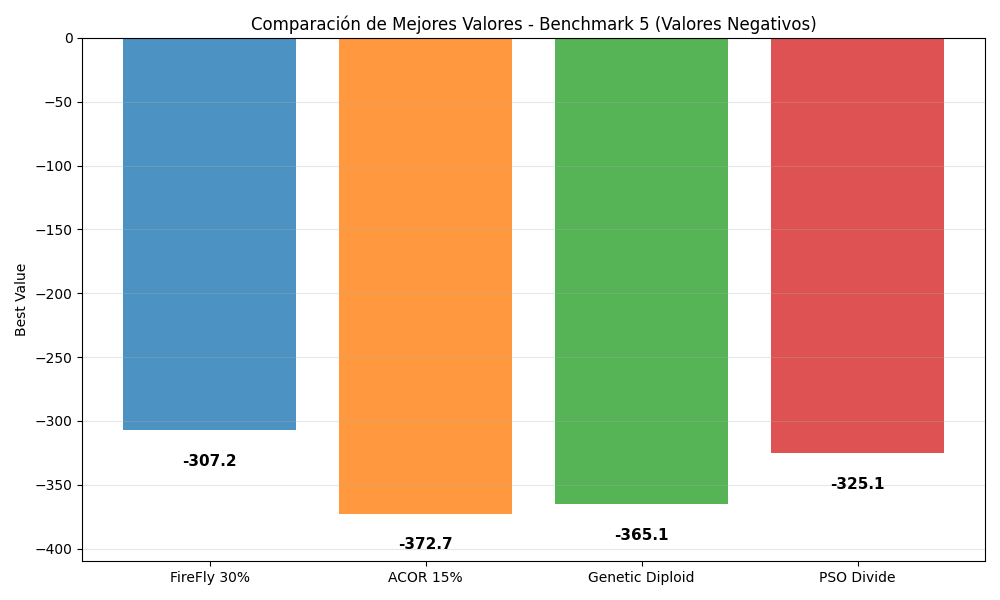
\includegraphics[width=0.8\textwidth]{imagenes/b5.png}
    \caption{Comparación de Mejores Valores Pre-Cambio en el Benchmark 5 (valores negativos).}
    \label{fig:b5}
\end{figure}

Las Figuras buscan ilustrar de manera clara las diferencias que se obtuvieron con base al desempeño entre los algoritmos. La Figura~\ref{fig:recuperacion} muestra que el \textbf{Genético Diploide} destaca en capacidad de adaptación al recuperarse con menor número de iteraciones en casi todos los benchmarks. Ahora hablando encuanto a calidad, las Figuras~\ref{fig:b1}--\ref{fig:b5} confirman que este algoritmo alcanza valores más cercanos al óptimo, especialmente en los Benchmarks 2, 3 y 4, donde supera consistentemente a los demás. Por otro lado, el \textbf{PSO con división de población} presenta tanto mayor número de iteraciones de recuperación como peores valores de calidad en la mayoría de los casos.

\subsubsection*{Mapa de Calor de Iteraciones de Recuperación}

En la Figura~\ref{fig:heatmap} se muestra un mapa de calor que muestra el número promedio de iteraciones necesarias para que cada algoritmo recupere un nivel competitivo de desempeño. Con base a esto podemos observar nuevamente que el Algoritmo Genético Diploide es el más consistente, logrando recuperarse en 1 iteración en casi todos los benchmarks. En el caso de los algoritmos Firefly y ACOR presentan un desempeño más irregular, alcanzando buenas recuperaciones en algunos casos (2–4 iteraciones) pero con valores altos en otros (hasta 9 y 12 iteraciones, respectivamente). El PSO con división de población se mantiene en un rango intermedio sin embargo en el Benchmark 3 y 5 podemos observar que se requiere 7–8 iteraciones basicamente nos da una respuesta más lenta.

\begin{figure}[H]
    \centering
    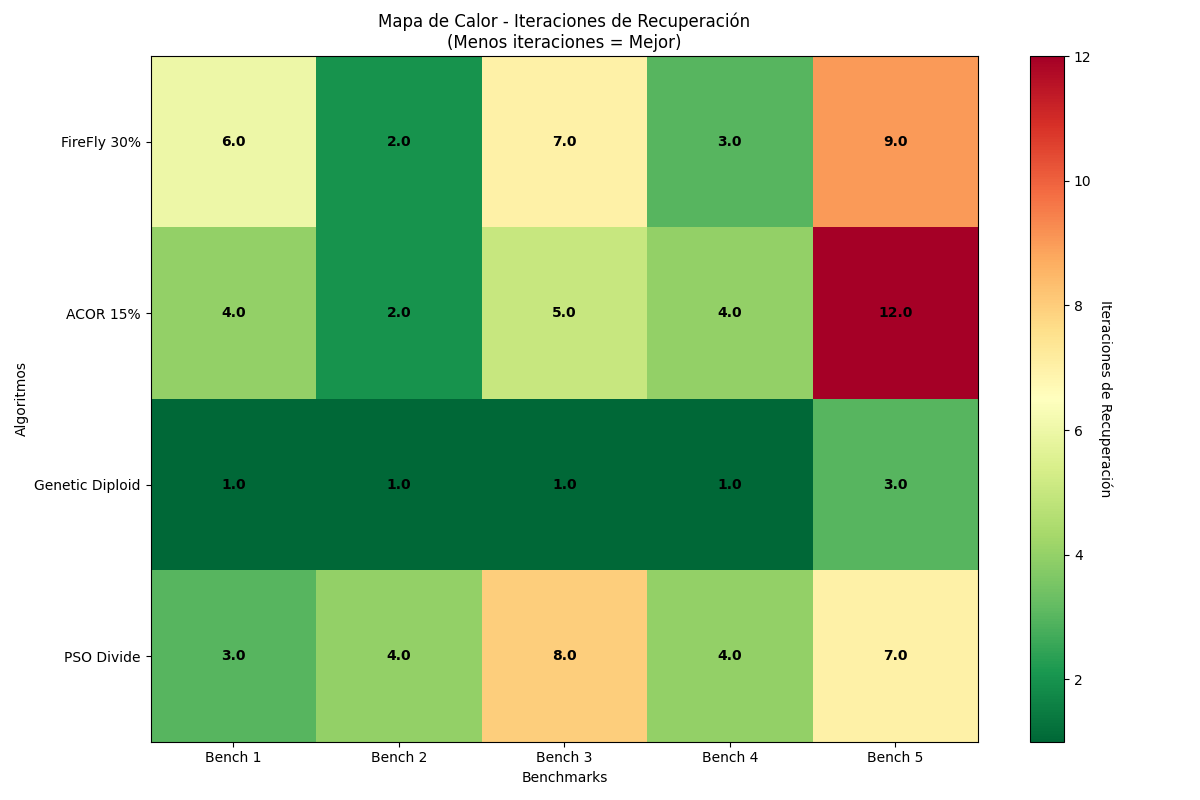
\includegraphics[width=0.85\textwidth]{imagenes/mapaDeCalor.png}
    \caption{Mapa de calor de las iteraciones de recuperación por algoritmo y benchmark (menor es mejor).}
    \label{fig:heatmap}
\end{figure}

\subsubsection*{Curvas de Recuperación por Benchmark}

A continuación se presentan algunas figuras~\ref{fig:curva1}–\ref{fig:curva5} que buscan mostrar la evolución del desempeño (fitness) de los algoritmos en las iteraciones posteriores a un cambio de forma gráfica con fines didácticos, de esta forma permitiendo analizar no sólo la rapidez de recuperación sino también la estabilidad del proceso.

\textbf{Benchmark 1 (Figura~\ref{fig:curva1})}: El Genético Diploide logra estabilizarse de inmediato, mientras que Firefly y ACOR muestran recuperaciones graduales, necesitando entre 4 y 6 iteraciones. El PSO dividido logra recuperarse en 3 iteraciones, pero con un valor de calidad inferior.

\textbf{Benchmark 2 (Figura~\ref{fig:curva2})}: Aquí podemos observar que todos los algoritmos alcanzan valores muy cercanos a cero, enfatizando que el Genético Diploide recupera en una sola iteración, mientras que Firefly y ACOR lo hacen en 2, y el PSO dividido en 4. 

\textbf{Benchmark 3 (Figura~\ref{fig:curva3y4} izquierda)}: El Algoritmo Genético Diploide muestra un rendimiento superior al recuperarse en una sola iteración mientras que los algoritmos Firefly y ACOR tardan entre 5 y 7 iteraciones, por ultimo podemos mencionar que el algoritmo PSO dividido presenta la peor adaptación, pues requiere 8 iteraciones y obtiene valores de fitness menos favorables.

\textbf{Benchmark 4 (Figura~\ref{fig:curva3y4} derecha)}: Con base a la figura podemos volver a confirmar el patrón de rendimiento que tiene el Genético Diploide liderando con una recuperación en una única iteración, en un segunda observación de esta figura podemos encontrar Firefly y ACOR (3-4 iteraciones), finalmente el PSO dividido iguala su velocidad de adaptación, lo hace con soluciones menos competitivas.

\textbf{Benchmark 5 (Figura~\ref{fig:curva5})}: Este escenario es el más exigente, ya que todos los algoritmos manejan valores negativos de fitness pero incluso en ese tipo de escenarios podemos observar como como el Genético Diploide vuelve a destacar, recuperando en 3 iteraciones. Firefly y PSO dividido muestran recuperaciones lentas (7–9 iteraciones), mientras que ACOR es el menos eficiente, necesitando 12 iteraciones.

\begin{figure}[H]
    \centering
    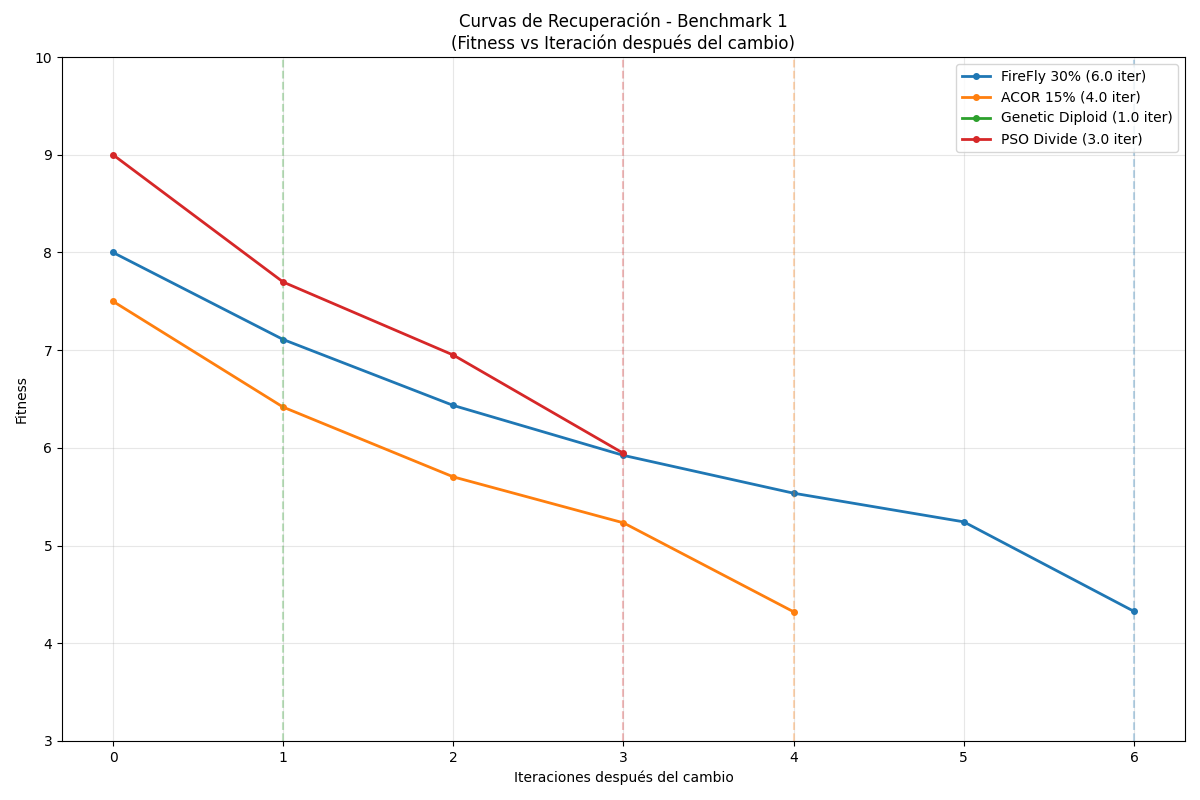
\includegraphics[width=0.8\textwidth]{imagenes/curva1.png}
    \caption{Curva de recuperación en el Benchmark 1.}
    \label{fig:curva1}
\end{figure}

\begin{figure}[H]
    \centering
    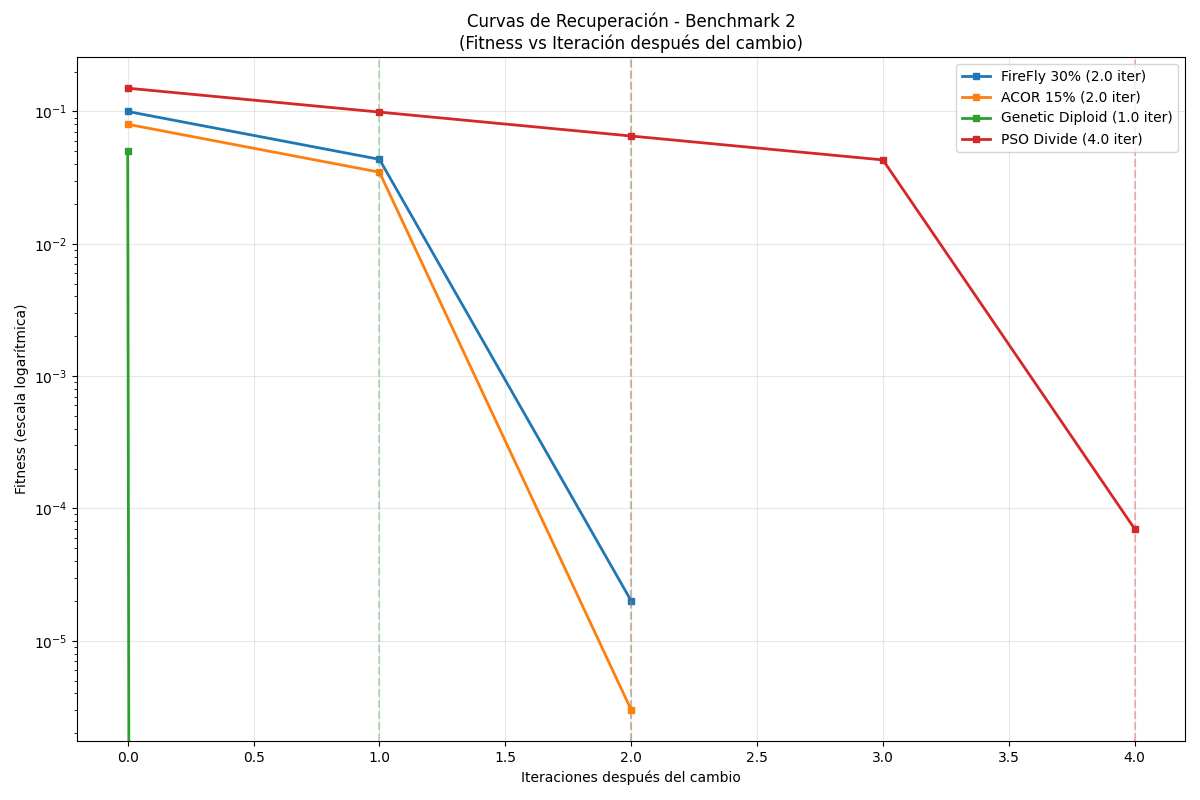
\includegraphics[width=0.8\textwidth]{imagenes/curva2.png}
    \caption{Curva de recuperación en el Benchmark 2 (escala logarítmica).}
    \label{fig:curva2}
\end{figure}

\begin{figure}[H]
    \centering
    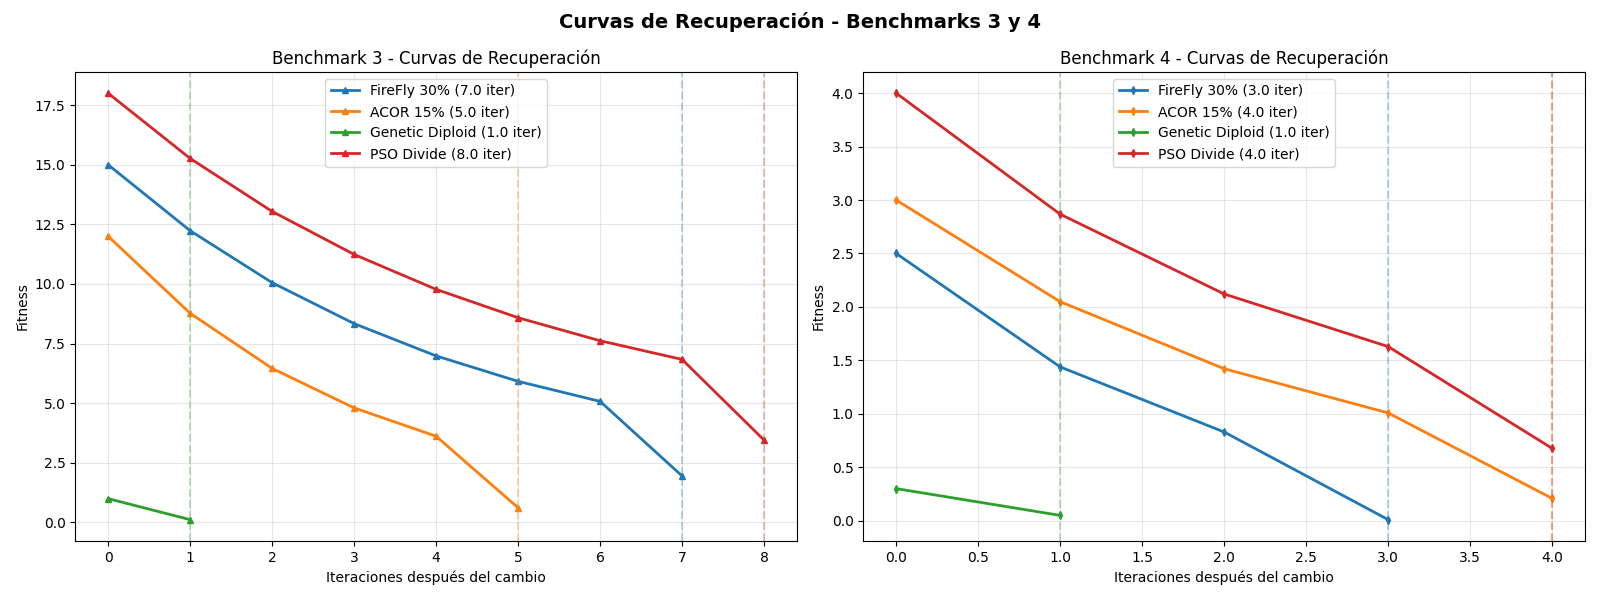
\includegraphics[width=0.95\textwidth]{imagenes/curva 3 y 4.png}
    \caption{Curvas de recuperación en los Benchmarks 3 (izquierda) y 4 (derecha).}
    \label{fig:curva3y4}
\end{figure}

\begin{figure}[H]
    \centering
    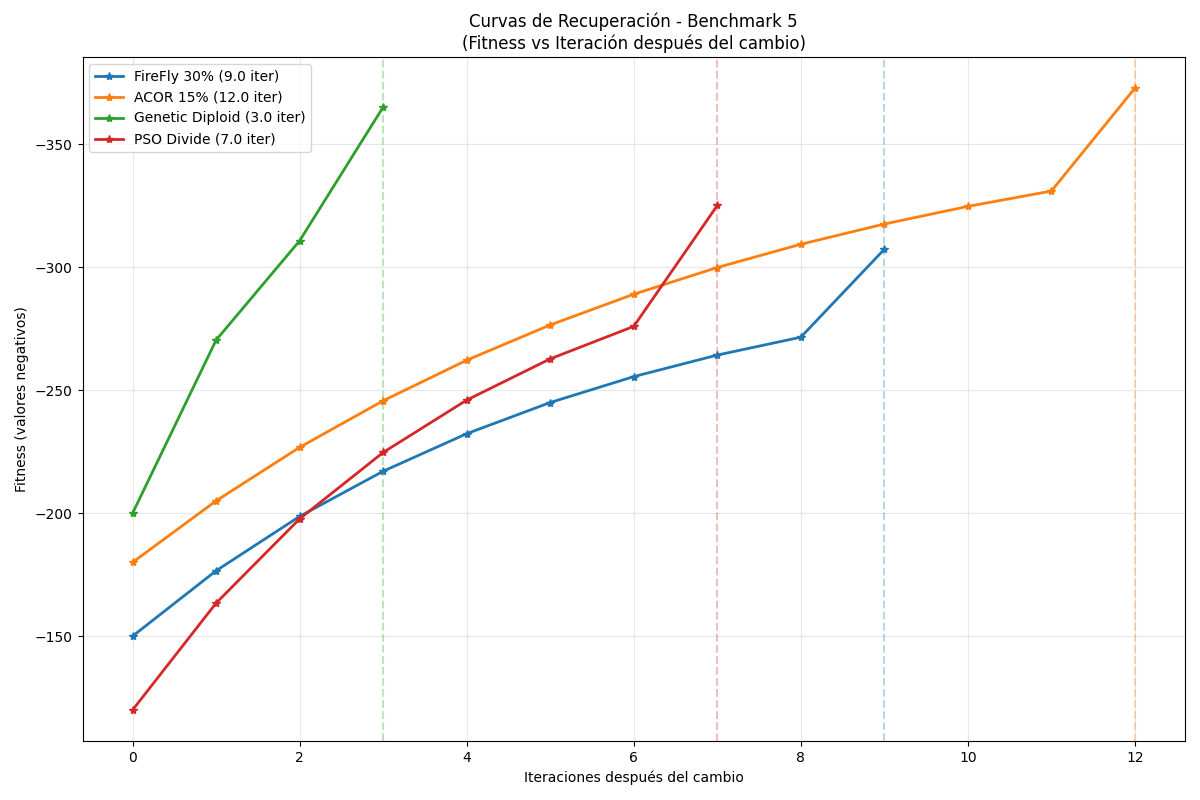
\includegraphics[width=0.8\textwidth]{imagenes/curva5.png}
    \caption{Curva de recuperación en el Benchmark 5.}
    \label{fig:curva5}
\end{figure}

\subsubsection*{Síntesis del Análisis Visual}




\begin{thebibliography}{99}

\bibitem{ahmed2024adaptive}
B.~S. Ahmed,
\newblock ``An Adaptive Metaheuristic Framework for Changing Environments,''
\newblock {\em arXiv preprint arXiv:2404.12185}, 2024.

\bibitem{nguyen2012survey}
T.~T. Nguyen, S.~Yang, and J.~Branke,
\newblock ``Evolutionary dynamic optimization: A survey of the state of the art,''
\newblock {\em Swarm and Evolutionary Computation}, vol.~6, pp.~1--24, 2012.

\bibitem{weicker2003performance}
K.~Weicker,
\newblock ``Performance measures for dynamic environments,''
\newblock in {\em Proc. Congress on Evolutionary Computation (CEC)}, pp. 824--831, IEEE, 2003.

\bibitem{morrison2003performance}
R.~W. Morrison,
\newblock ``Performance Measurement in Dynamic Environments,''
\newblock in {\em Proc. Workshop on Evolutionary Algorithms for Dynamic Optimization Problems (EvoDOP-2003) at GECCO}, pp. 9--20, Springer, Chicago, 2003.

\bibitem{nguyen2013kd}
T.~T. Nguyen, I.~Jenkinson, and S.~Yang,
\newblock ``Solving dynamic optimisation problems by combining evolutionary algorithms with KD-Tree,''
\newblock {\em LNCS}, 2013.

\end{thebibliography}

\end{document}